\hypertarget{introduction}{%
\section{Introduction}\label{introduction}}

This comprehensive report delves into the performance analysis of a heat
simulation application, deployed on diverse hardware setups. We
scrutinize the application on Yggdrasil High-Performance Computing (HPC)
with an array of 32 CPUs and a GPU, juxtaposed against its performance
on a personal computer equipped with 12 CPU cores and an NVIDIA RTX 2070
Super GPU. The crux of this analysis lies in discerning the execution
time disparities when run on CPU versus GPU.

\hypertarget{methodology}{%
\section{Methodology}\label{methodology}}

\hypertarget{hardware-employed}{%
\subsection{Hardware Employed}\label{hardware-employed}}

\begin{itemize}
\tightlist
\item
  \textbf{Yggdrasil HPC:} A formidable configuration of 32 CPUs
  alongside a single GPU.
\item
  \textbf{Personal Computer:} A setup comprising 12 CPU cores and an RTX
  2070 Super GPU.
\end{itemize}

\hypertarget{software-and-compilation}{%
\subsection{Software and Compilation}\label{software-and-compilation}}

\begin{itemize}
\tightlist
\item
  The application is compiled using \texttt{g++} for CPU-centric
  execution, and \texttt{nvcc}, NVIDIA's CUDA compiler, for GPU
  execution.
\item
  The incorporation of the Threading Building Blocks (TBB) library
  (\texttt{-ltbb}) hints at the application's potential for
  multi-threaded operations on the CPU.
\end{itemize}

\hypertarget{results}{%
\section{Results}\label{results}}

\hypertarget{performance-metrics}{%
\subsection{Performance Metrics}\label{performance-metrics}}

\begin{enumerate}
\def\labelenumi{\arabic{enumi}.}
\tightlist
\item
  \textbf{On Yggdrasil HPC:}

  \begin{itemize}
  \tightlist
  \item
    \textbf{CPU (32 cores):} Marked an execution time of 4,139,176
    microseconds.
  \item
    \textbf{GPU:} Recorded an execution time of 5,800,258 microseconds.
  \end{itemize}
\item
  \textbf{On Personal Computer:}

  \begin{itemize}
  \tightlist
  \item
    \textbf{CPU (12 cores):} Notched an execution time of 2,653,190
    microseconds.
  \item
    \textbf{GPU (RTX 2070 Super):} Clocking in at 2,652,420
    microseconds.
  \end{itemize}
\end{enumerate}

\hypertarget{graphical-representation}{%
\section{Graphical Representation}\label{graphical-representation}}

A bar graph vividly depicts the execution times, contrasting the
performance across the varied hardware configurations.

\begin{figure}
\centering
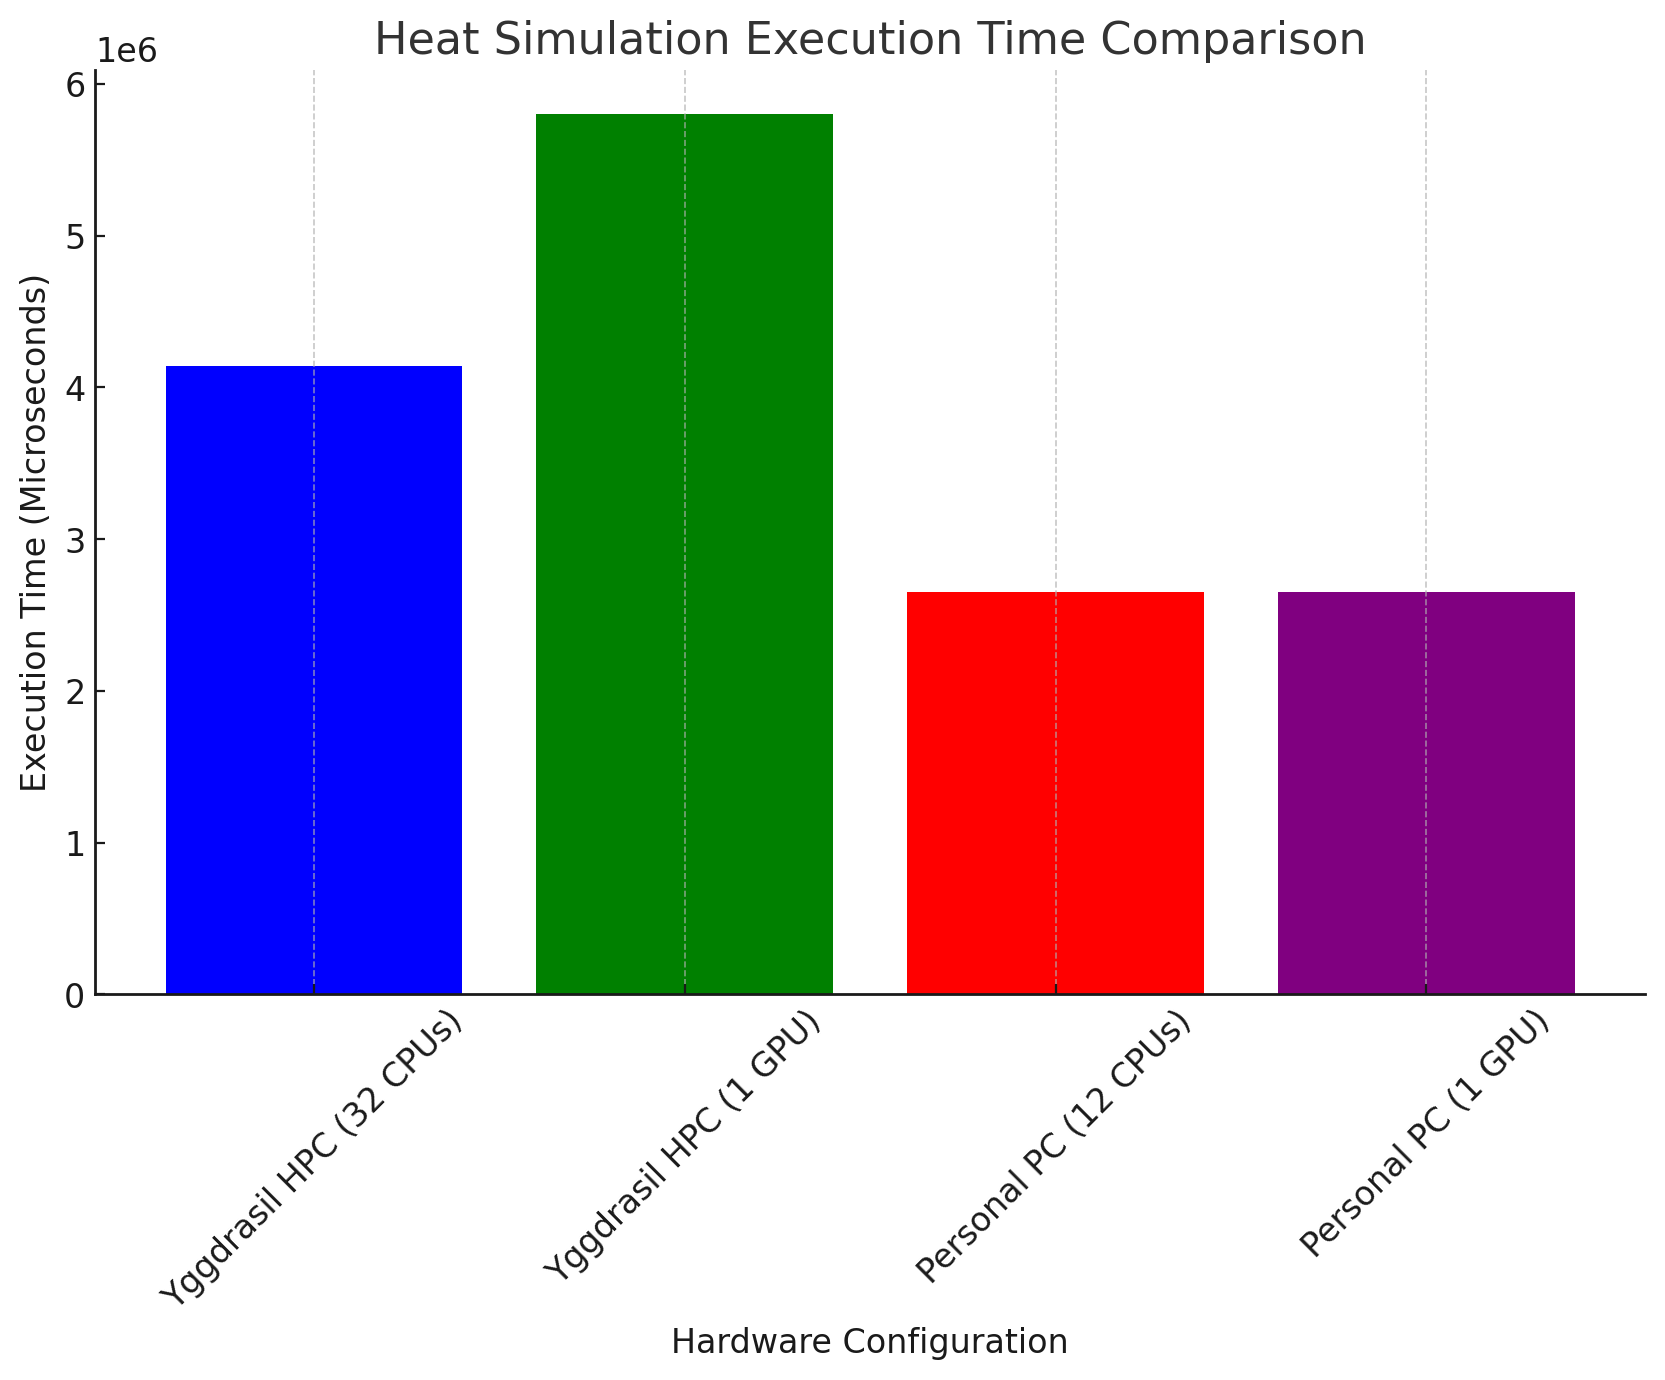
\includegraphics{img/execution_time.png}
\caption{Execution Times}
\end{figure}

\hypertarget{analysis-of-code}{%
\section{Analysis of Code}\label{analysis-of-code}}

\hypertarget{cpu-implementation}{%
\subsection{CPU Implementation}\label{cpu-implementation}}

\begin{itemize}
\tightlist
\item
  The code harnesses an array of standard C++ libraries for various
  functionalities, ranging from input/output operations to mathematical
  computations and parallel execution capabilities.
\item
  Key constants like \texttt{max\_iter}, \texttt{Nx}, and \texttt{Ny}
  are pivotal in setting the simulation parameters.
\item
  The vectors \texttt{U} and \texttt{U0} are instrumental in
  representing the state of the simulation grid.
\item
  The simulation loop leverages \texttt{std::for\_each} combined with
  \texttt{std::execution::par\_unseq}, optimizing for parallel execution
  across CPU cores.
\item
  Timing metrics are meticulously captured using
  \texttt{high\_resolution\_clock}, providing granular insights into
  execution efficiency.
\end{itemize}

\hypertarget{gpu-implementation}{%
\subsection{GPU Implementation}\label{gpu-implementation}}

\begin{itemize}
\tightlist
\item
  The specifics of GPU optimization and parallel processing remain
  elusive in the provided code snippet, leaving room for speculation
  about its execution efficiency and optimization on the GPU front.
\end{itemize}

\hypertarget{discussion}{%
\section{Discussion}\label{discussion}}

\hypertarget{performance-insights}{%
\subsection{Performance Insights}\label{performance-insights}}

\begin{itemize}
\tightlist
\item
  \textbf{Personal Computer:} The performance metrics interestingly
  reveal that the GPU, despite having fewer cores than the CPU, delivers
  comparable execution efficiency.
\item
  \textbf{Yggdrasil HPC:} The CPU's performance notably eclipses that of
  the GPU, indicating more effective utilization of resources or
  possibly superior parallel processing capabilities in this scenario.
\end{itemize}

\hypertarget{factors-influencing-performance}{%
\subsection{Factors Influencing
Performance}\label{factors-influencing-performance}}

\begin{itemize}
\tightlist
\item
  \textbf{CPU Efficiency:} The application's CPU version exhibits
  impressive multi-threading efficiency, particularly on the HPC's
  multi-core setup.
\item
  \textbf{GPU Limitations:} GPU performance could be hindered by factors
  like memory transfer bottlenecks and less optimized kernel execution,
  particularly evident in the HPC environment.
\end{itemize}

\hypertarget{potential-for-optimization}{%
\subsection{Potential for
Optimization}\label{potential-for-optimization}}

\begin{itemize}
\tightlist
\item
  Both CPU and GPU implementations present opportunities for
  enhancement. Optimizing memory access patterns, refining thread
  management, and fine-tuning kernel execution parameters for GPUs are
  potential areas for improvement.
\end{itemize}

\hypertarget{conclusion}{%
\section{Conclusion}\label{conclusion}}

The report meticulously evaluates the performance of a heat simulation
application across various hardware settings, uncovering valuable
insights into its operational dynamics. The findings gleaned from this
analysis serve as a cornerstone for strategizing optimizations tailored
to high-performance computing applications.
